\documentclass{standalone}
\usepackage{tikz}
\usepackage{ctex,siunitx}
\setCJKmainfont{Noto Serif CJK SC}
\usepackage{tkz-euclide}
\usepackage{amsmath}
\usetikzlibrary{patterns, calc,3d}
\usetikzlibrary {decorations.pathmorphing,decorations.pathreplacing,decorations.shapes}
\tikzset{
  every node/.style={circle,thick,draw=red!50!black,fill=red!20!white,minimum height=7mm}
}
\begin{document}
\small
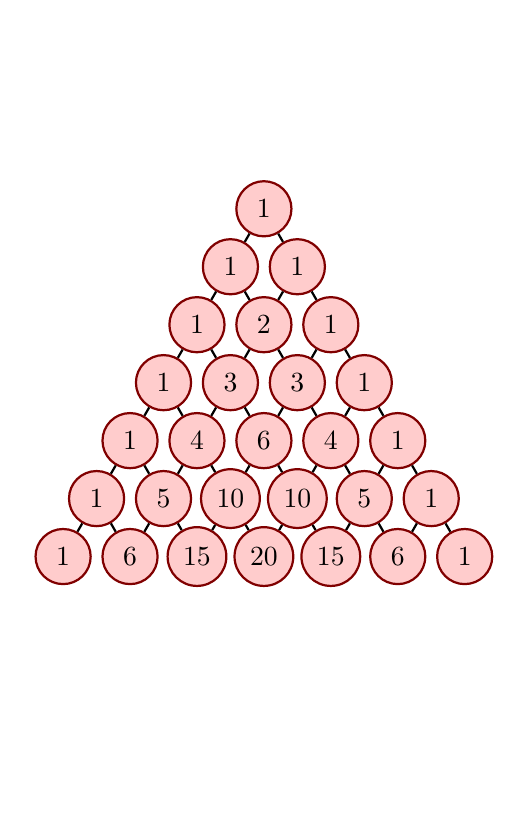
\begin{tikzpicture}[>=latex,scale=1.0]
  \useasboundingbox(-3,-7.6)rectangle(3,2.3);
  \begin{scope}[scale=0.85]
  \node (00) at (0,0){1};
  \node (10) at (-120:1){1};
  \node (11) at (-60:1){1};
  \foreach \x[count =\i from 0] in {1,2,1}
  {
    \node(2\i) at ([xshift=\i cm]-120:2){\x};
  }
  \foreach \x[count =\i from 0] in {1,3,3,1}
  {
    \node(3\i) at ([xshift=\i cm]-120:3){\x};
  }
  \foreach \x[count =\i from 0] in {1,4,6,4,1}
  {
    \node(4\i) at ([xshift=\i cm]-120:4){\x};
  }
  \foreach \x[count =\i from 0] in {1,5,10,10,5,1}
  {
    \node(5\i) at ([xshift=\i cm]-120:5){\x};
  }
  \foreach \x[count =\i from 0] in {1,6,15,20,15,6,1}
  {
    \node(6\i) at ([xshift=\i cm]-120:6){\x};
  }
  \draw[thick]
  (00)--(10)--(20)--(30)--(40)--(50)--(60)
  (00)--(10)--(20)--(30)--(40)--(50)--(60)
  (00)--(11)--(22)--(33)--(44)--(55)--(66)
  (11)--(21)--(31)--(41)--(51)--(61)
  (10)--(21)--(32)--(43)--(54)--(65)
  (20)--(31)--(42)--(53)--(64)
  (22)--(32)--(42)--(52)--(62)
  (30)--(41)--(52)--(63)
  (33)--(43)--(53)--(63)
  (40)--(51)--(62)
  (44)--(54)--(64)
  (50)--(61)
  (55)--(65)
  ;
  \end{scope}
\end{tikzpicture}
\end{document}